% Document class and font size
\documentclass[a4paper,10pt]{extarticle}

% Packages
\usepackage[utf8]{inputenc} % For input encoding
\usepackage{geometry} % For page margins
\geometry{a4paper, margin=0.75in} % Set paper size and margins
\usepackage{titlesec} % For section title formatting
\usepackage{enumitem} % For itemized list formatting
\usepackage{hyperref} % For hyperlinks
\usepackage{kotex}
\usepackage{graphicx}
\usepackage{array}
\usepackage{longtable}

% Formatting
\setlist{noitemsep} % Removes item separation
\titleformat{\section}{\large\bfseries}{\thesection}{1em}{}[\titlerule] % Section title format
\titlespacing*{\section}{0pt}{\baselineskip}{\baselineskip} % Section title spacing
\graphicspath{{pictures}}

% Begin document
\begin{document}
% Disable page numbers
\pagestyle{empty}
% Enable page numbers
% \pagenumbering{arabic}

% Header

% \begin{minipage}{\textwidth}

\begin{minipage}{0.1\textwidth}
    \begin{flushleft}
        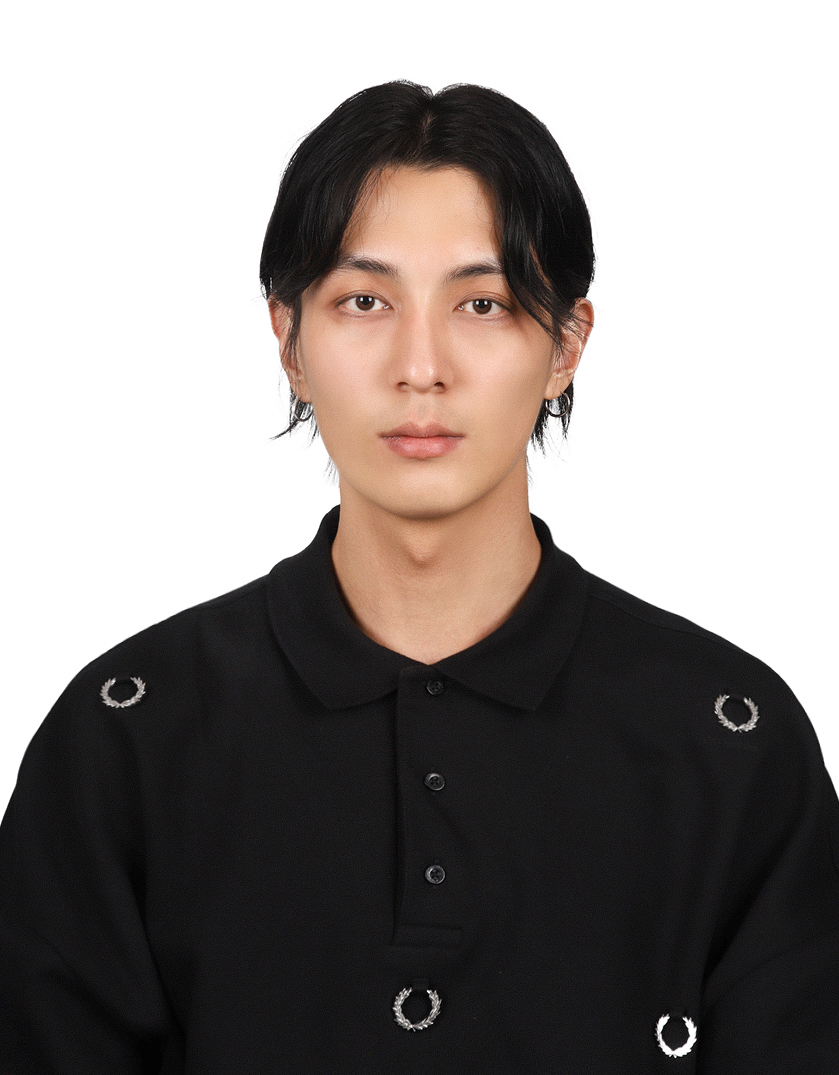
\includegraphics[height=3.5cm]{photo_231008.jpeg}
    \end{flushleft}
\end{minipage}
\hfill
\begin{minipage}{0.7\textwidth}
    \begin{flushright}
        \textbf{\Large Hyeonbeen Lee} % Name
        \newline\newline
        \begin{tabular}{rl}
            \textbf{Mobile: }   & +82-10-6236-4693                                                                                     \\
            \textbf{EMail: }    & \href{mailto:david.hyeonbeen.lee@gmail.com}{david.hyeonbeen.lee@gmail.com}                           \\
            % \textbf{Instagram: } & \href{https://www.instagram.com/leehyeonbeen}{@leehyeonbeen}                                         \\
            \textbf{LinkedIn: } & \href{https://www.linkedin.com/in/hyeonbeen-lee-239500286/}{linkedin.com/in/hyeonbeen-lee-239500286} \\
            \textbf{GitHub: }   & \href{https://github.com/hyeonbeenlee}{github.com/hyeonbeenlee}                                      \\
        \end{tabular}
        % \end{center}
    \end{flushright}

\end{minipage}
% \end{minipage}


% Education Section
\newcolumntype{L}{>{\raggedright\arraybackslash}m{3.5cm}}
\newcolumntype{R}{>{\centering\arraybackslash\small}m{4cm}}
\renewcommand*{\arraystretch}{1.5}
\noindent
\section*{PERSONAL INFORMATION}
\begin{center}
    \vspace*{-0.8cm}
    \noindent
    \begin{longtable}{LRLRLR}
        \textbf{Name:}             & Hyeonbeen Lee                                                                          & \textbf{Date of birth:}     & July 4th, 1996                                              \\
        \hline
        \textbf{Nationality:}      & Republic of Korea (South)                                                              & \textbf{Address:}           & 116, Saimdang-ro 17gil, Seoul, South Korea                  \\
        \hline
        \textbf{Military service:} & Honorably discharged,\linebreak Marine Corps Seageant \small{(May 2017$\sim$Feb 2019)} & \textbf{Research interest:} & Robot learning, Reinforcement learning, Sequential decision \\
        \hline
    \end{longtable}
\end{center}

% Education Section
\section*{EDUCATION}
\noindent
\textbf{Banpo High School}, Science Immersed Track \hfill Mar 2012 | Feb 2015
\newline
\textbf{Kyung Hee University}, Dept. of Mechanical Engineering \hfill Mar 2015 | Feb 2022\\ % University name and location
Bachelor's Degree (Supervisor: Shin-kyu Jeong, Jin-gyun Kim)\hfill GPA: 3.87/4.5, GPA(Major): 3.84/4.5\\ % Degree and GPA
Thesis: \textit{\small{Data-driven aerodynamic coefficient prediction using}}\\
\hspace*{1.3cm}\textit{\small{deep neural
        network and PARSEC airfoil parameterization}}
\newline
\textbf{Kyung Hee University}, Dept. of Mechanical Engineering \hfill Mar 2022 | Feb 2024\\ % University name and location
Master's Degree (Supervisor: Jin-gyun Kim) \hfill GPA: 4.33/4.5\\ % Degree and GPA
Thesis: \textit{\small{Composite neural network with differential propagation}}\\
\hspace*{1.3cm}\textit{\small{for modeling impulsive nonlinear dynamic systems}}

\section*{SKILLS}
\begin{itemize}
    \item \textbf{Programming: }Python, Docker, Linux, Git, \LaTeX, MATLAB, C\#, C++, ROS
    \item \textbf{ML and data analysis:} PyTorch, TensorBoard, Pandas, OpenCV, Torchvision
    \item \textit{Expertised at handling \underline{sequential data and models}}
    \item \textbf{English: }Speaks in native level
    \item \textbf{Japanese: }Speaks in intermediate level
\end{itemize}


Experience Section
\section*{PUBLICATIONS}
\noindent
\begin{enumerate}[leftmargin=.5cm]
    \item S. Han, G.E. Jeong, \textbf{H. Lee}, W.S. Choi, J.G. Kim, “Multi-body dynamics model for spent nuclear fuel transportation system under normal transport test conditions”, \textit{Nuclear Engineering and Technology} (IF=2.817), accepted.
    \item \textbf{H. Lee}, S. Han, H.S. Choi, J.G. Kim. “cNN-DP: Composite neural network with differential propagation for impulsive nonlinear dynamics”, \textit{Journal of Computational Physics (IF=4.645)}, submitted.
    \item \textbf{H. Lee}, J. Han, T. Yeo, J.G. Kim. “Multi-horizon force components forecasting of ocean robot using interpretable Transformer and experimental measurements”, in preparation.
\end{enumerate}

% Experience Section
\section*{CONFERENCES}
\noindent
\newcolumntype{L}{>{\raggedright\arraybackslash}m{3.4cm}}
\newcolumntype{R}{>{\raggedright\arraybackslash}m{13.2cm}}
\vspace*{-.5cm}
\begin{longtable}{LR}
    {2022.12.04 \linebreak Jeju, South Korea}    & \textbf{H. Lee}, S. Han, G.E. Jeong, J.G. Kim. “Development of multibody dynamics trailer model using normal transportation test data and DNN based surrogate model generation”, Fall conference, Korean Society for Noise and Vibration Engineering (Oral Presentation). \\
    {2023.02.16 \linebreak  Austin, Texas, USA}  & \textbf{H. Lee,} S. Han, H.S. Choi, J.G. Kim. “Composite neural network framework for modeling impulsive nonlinear dynamic responses”, IMAC-XLI, Society for Experimental Mechanics (Oral Presentation).                                                                  \\
    {2023.03.23 \linebreak Jeju, South Korea}    & \textbf{H. Lee,} S. Han, H.S. Choi, J.G. Kim. “Meta-modeling of nonlinear impulsive dynamics using composite neural network model with differential propagation”, Conference on Dynamics and Control, Korean Society of Mechanical Engineers (Oral Presentation).         \\
    {2023.05.18 \linebreak Busan, South Korea}   & \textbf{H. Lee,} S. Han, H.S. Choi, J.G. Kim. “Meta-modeling of nonlinear impulsive dynamics using composite neural network model with differential propagation”, Conference on Engineering Reliability, Korean Society of Mechanical Engineers (Oral Presentation).      \\
    {2023.11.01 \linebreak Incheon, South Korea} & \textbf{H. Lee}, J. Han, T. Yeo, J.G. Kim. “Real-time multi-horizon reaction force forecasting of ocean robot using interpretable Transformer”, Annual Conference, Korean Society of Mechanical Engineers (Oral Presentation).                                            \\
\end{longtable}


% Experience Section
\section*{PROJECTS}
\noindent
\newcolumntype{L}{>{\raggedright\arraybackslash}m{3cm}}
\newcolumntype{R}{>{\raggedright\arraybackslash}m{14cm}}
\vspace*{-.5cm}
\begin{longtable}{LR}
    {2021.09 | 2022.10} & Development of ground·sea transportation test simulation model using multibody dynamics and DNN-based metamodel, Korea Atomic Energy Research Institute (KAERI).                                                                                                                                                                                   \\
    {2021.09 | Present} & Metamodel generation and evolution procedures for flexible multibody dynamics, FunctionBay Inc.                                                                                                                                                                                                                                                    \\
    {2021.11 | Present} & cNN-DP: Composite neural network with differential propagation for impulsive nonlinear dynamics, Modeling \& Simulation Lab. (\href{https://github.com/hyeonbeenlee/cNN-DP}{github.com/hyeonbeenlee/cNN-DP})                                                                                                                                       \\
    {2022.03 | Present} & Deep-learning based reaction force and torque prediction model development for underwater ground cutting robot using experimental measurements and dynamic simulation data, Korea Research Institute of Ships and Ocean Engineering (KRISO). (\href{https://github.com/hyeonbeenlee/TimeSeriesSeq2Seq}{github.com/hyeonbeenlee/TimeSeriesSeq2Seq}) \\
    {2022.12 | 2023.06} & RecurDyn Automation using Python, Modeling \& Simulation Lab. (\href{https://github.com/hyeonbeenlee/RecurDynPython}{github.com/hyeonbeenlee/RecurDynPython})                                                                                                                                                                                      \\
    {2023.03 | 2023.06} & Segment Anyone: Fine-tuned Segment-Anything-Model (SAM) for human-collaborative robots, Kyung Hee University Dept. of Artifical Intelligence. (\href{https://github.com/hyeonbeenlee/segment-anything-fine-tuning}{github.com/hyeonbeenlee/segment-anything-fine-tuning})                                                                          \\
\end{longtable}

% Skills Section
\section*{AWARDS AND CERTIFICATES}
\begin{itemize}
    \item \textbf{TOEIC:} 925/990 \hfill No.605083, Nov 25 2018
    \item \textbf{New TEPS:} 513/600 \hfill No.0111736, May 13 2023
          % \item \textbf{제1종보통 운전면허} \hfill 경기도남부경찰청장, 취득번호: 13-22-624421-XX, 취득일: 2022.04.18
    \item \textbf{Academic Excellence Scholarship (Full tuition)} \hfill Kyung Hee University, Mar 01 2021
          % \item \textbf{행정조교 장학금} \hfill 경희대학교 대학원, 수혜년월: 2022.09 | 2024.02
    \item \textbf{Exellence Paper Award} \hfill Korean Society of Mechanical Engineers, No.2023-083, Aug 25 2023
\end{itemize}

% Experience Section
% \section*{사회경험}
% \noindent
% \textbf{맥도날드 서울교대점} 고객응대, 주방보조, 계산 \hfill 2014.11 - 2015.02\\
% \textbf{육회한연어 수원영통점} 서빙, 주방보조, 계산 \hfill 2016.02 - 2016.06\\
% \textbf{슈펜 가로수길점} 외국인 고객응대, 물류창고정리 \hfill 2016.06 - 2016.09\\
% \textbf{오늘 와인한잔 수원역점} 서빙, 주방보조 \hfill 2016.09 - 2016.12\\
% \textbf{아이리스 BAR} 서빙, 주방보조, 고객응대 \hfill 2019.03 - 2019.06\\
% \textbf{대명GEC} 삼성전자 화성사업장 케이블 배선작업 \hfill 2019.07 - 2019.08\\

% Experience Section
\section*{MISCELLANEOUS}
\textbf{ROK-US Marine Corps Joint Operations Translator} \hfill 1st Marine Div., ROKMC, Sep 2017 | Feb 2019\\
\textbf{48th Student Council} \hfill Kyung Hee University College of Engineering, Feb 2019 | Jan 2020\\
\textbf{Undergraduate Research Internship} \hfill Modeling \& Simulation Lab, Jan 2021 | Feb 2022\\
\textbf{Seminar: AI, Data Driven Models\&ML} \hfill {\small National Agency Finite Element Methods and Standard}, Apr 2021\\
\textbf{Seminar: AI Summer School 2021} \hfill Korean Society of Mechanical Engineers, Aug 2021\\
\textbf{Teaching Assistant (System Dynamics)} \hfill Modeling \& Simulation Lab, Mar 2022 - Jun 2023\\
\textbf{Seminar: AI Summer School 2022} \hfill Korean Society of Mechanical Engineers, Aug 2022\\
\textbf{Representative Administrative Assistant} \hfill Kyung Hee University, Sep 2022 | Present\\
\textbf{Seminar: IAS18 Workshop\&Tutorials} \hfill {\small Intl. Conference on Intelligent Autonomous Systems}, Jul 2023\\

% End document
\end{document}